\documentclass[12pt]{article}
\usepackage{epsfig}
\usepackage{tikz}
\usepackage{mathtools, amsmath, amssymb}
\usepackage{qtree}
\usepackage{array, booktabs}
\usepackage{caption}
%\usepackage[margin=0.75in]{geometry}
\usepackage{amsfonts}
\usepackage{hyperref}
\hypersetup{
    colorlinks=true,
    citecolor=blue,
    linkcolor=blue,
    filecolor=blue,      
    urlcolor=blue,
    }
\usetikzlibrary{arrows,shapes,decorations,automata,positioning,backgrounds,petri,tikzmark,calc}
\usepackage[
  authordate,
  backend=biber
]{biblatex-chicago}
\addbibresource{references.bib}

\usepackage{pifont}
\usepackage{utfsym}

\usepackage{pgfplots}
\pgfplotsset{compat=1.18}
\usepackage[section]{placeins}

% numeric sets
\newcommand{\Reals}{\mathbb{R}}      % real numbers
\newcommand{\Naturals}{\mathbb{N}}   % natural numbers
\newcommand{\Integers}{\mathbb{Z}}   % integer numbers
\newcommand{\Rationals}{\mathbb{Q}}  % rational numbers
\newcommand{\Complexes}{\mathbb{C}}  % complex numbers

% logic
\newcommand{\yields}{\vdash}         % yields
\newcommand{\proves}{\vdash}         % proves
\newcommand{\then}{\rightarrow}      % implication
\newcommand{\logeq}{\Leftrightarrow} % logically equivalent
% formal logic
\newcommand{\Models}{\vDash}                 % models
\newcommand{\Always}{\Box}                   % always
\newcommand{\Eventually}{\lozenge}           % eventually
\newcommand{\Next}{\mathcal{X}}              % ne[X]t
\newcommand{\Until}{\ \mathcal{U}\ }         % [U]ntil
\newcommand{\Release}{\ \mathcal{R}\ }       % [R]lease
\newcommand{\WeakUntil}{\ \mathcal{W}\ }     % [W]eak until
\newcommand{\MightyRelease}{\ \mathcal{M}\ } % [M]ighty release
\newcommand{\Globally}{\mathcal{G}}          % [G]lobally
\newcommand{\Finally}{\mathcal{F}}           % [F]inally
\newcommand{\ForAllPaths}{\mathcal{A}}       % for [A] paths
\newcommand{\ExistsAPath}{\mathcal{E}}       % exists a path

\newcommand{\overbar}[1]{\mkern 1.5mu\overline{\mkern-1.5mu#1\mkern-1.5mu}\mkern 1.5mu}

\listfiles

\title{\bf
\large Formal Verification of the MESI Cache Coherency Protocol using SPIN}
\author{Luke Marzen\\
\texttt{ljmarzen@iastate.edu}}
\date{December 13, 2023}

\renewcommand{\baselinestretch}{1.1}
\renewcommand{\arraystretch}{1.2}
\renewcommand{\dbltopfraction}{0.9}
\renewcommand{\topfraction}{0.9}
\renewcommand{\bottomfraction}{0.9}
\renewcommand{\dblfloatpagefraction}{0.99}
\renewcommand{\floatpagefraction}{0.99}
\renewcommand{\textfraction}{0.01}

\newcommand{\N}{\mathbb{N}}
\newcommand{\strings}{\{0, 1\}^\ast}
\newcommand{\dom}{\text{{\it dom} }}
\newcommand{\range}{\text{{\it range}}}
\newcommand{\sstrings}{\Sigma^\ast}
\newcommand{\pair}[2]{{<}#1,{#2}{>}}
\newcommand{\class}[1]{\mathcal{#1}}


\tikzset{fontscale/.style = {font=\relsize{#1}}}

\tikzstyle{startstop} = [rectangle, rounded corners, 
minimum width=1cm, 
minimum height=1cm,
text centered,
text width=2cm,
draw=black,
font = {\scriptsize},
fill=red!30]

\tikzstyle{io} = [trapezium, 
trapezium stretches=true, % A later addition
trapezium left angle=70, 
trapezium right angle=110,
minimum width=1cm, 
minimum height=1cm,
text centered, 
draw=black, fill=blue!30]

\tikzstyle{process} = [rectangle, 
minimum width=1cm, 
minimum height=1cm, 
text centered, 
text width=3cm,
draw=black, 
fill=violet!30]

\tikzstyle{decision} = [diamond, 
minimum width=1cm, 
minimum height=1cm, 
text centered, 
draw=black, 
fill=orange!30]
\tikzstyle{arrow} = [thick,->,>=stealth]


\begin{document}

\maketitle

% \thispagestyle{empty}

% \begin{abstract}
% \bf
% \end{abstract}

\section{Introduction}

Cache coherency is critical for maintaining a up-to-date view of memory between multiple processors. To achieve coherency, a protocol is employed. MESI is a widely-used cache coherency protocol. The aim of this project is to verify the MESI cache coherency protocol by employing \textit{Model Checking}. To this end, a parameterizable cache model is constructed in Promela to be verified in SPIN.

\subsection{Overview}

Background information is reviewed in Section \ref{background}. Section \ref{model} begins with an overview of the construction of the model, then discusses the validation efforts in Subsection \ref{model_validation}. Verification of the model is discussed in Subsection \ref{model_verification}. Results are presented in Section \ref{results} and conclusions are presented in Section \ref{conclusion}.

\section{Background} \label{background}

Processors have several levels of memory storage which are organized according to their proximity to the CPU and access-time. This concept is referred to as the \textit{Memory Hierarchy}. Memory hierarchies are motivated by practical constraints that prevent us from having indefinitely large memory with immediate access.

\subsection{Cache Coherency}

Modern multi-processor systems consist of multiple CPUs, each with their own registers and cache(s). Figure \ref{fig:cachediagram} illustrates this relationship. To maintain correct program execution for programs utilizing shared memory it is crucial that a \textit{coherent}, up-to-date, view of memory is maintained between all CPUs. A \textit{cache coherency protocol} describes the permitted transactions and how those changes are propagated to other caches in order to ensure the desired behavior is preserved. In section \ref{model_verification} we will define this more formally.

\begin{figure}[h!]
    \centering
    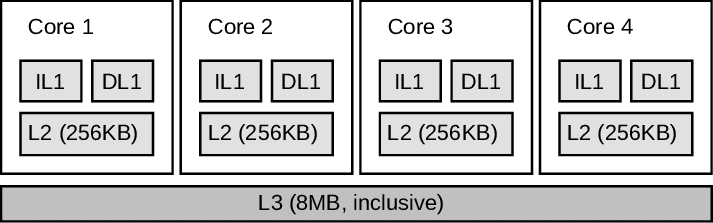
\includegraphics[width=10cm]{images/Intel-Core-i7-cache-architecture.png}
    \caption{Cache architecture of the Intel Core i7 4790 processor. (\cite{nakamoto2018})}
    \label{fig:cachediagram}
\end{figure}

\subsection{MESI}

\textit{MESI} is a popular cache coherency protocol originally proposed by (\cite{papamarcos1984}). The name itself is an acronym for the four states that a cache block can be assigned: \textit{Modified}, \textit{Exclusive}, \textit{Shared}, and \textit{Invalid}. The MESI protocol can be defined by a finite-automata shown in Figure \ref{fig:statetransitiondiagram}. Each private cache is connected to a \textit{caching-agent} (i.e. a processor) as well as a shared bus which is used to communicate state transitions.

\begin{figure}[h!]
    \centering
    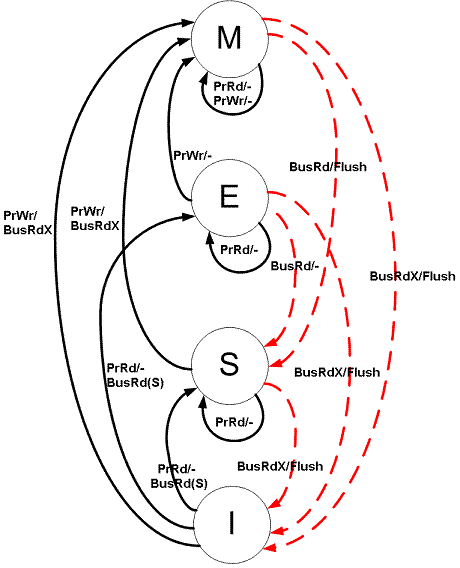
\includegraphics[height=8cm]{images/State_transition_diagram_for_the_Illinois_MESI_protocol.png}
    \caption{State transition diagram for Illinois MESI protocol. Transitions: Processor initiated transactions (black), Bus initiated transaction (red). (\cite{culler1998})}
    \label{fig:statetransitiondiagram}
\end{figure}

\subsection{Snooping}

Snooping is the first of two competing techniques used by cache coherency protocols to achieve communication of cache transactions and propagate state changes. This solution employs a shared interconnect or bus which cache transactions are broadcasted on to all other caches. Each caches is constantly monitoring or \textit{snooping} this shared bus and updated the state of its cache accordingly. Snooping protocols are typically only reserved for processors with small core counts since the shared bus quickly becomes a bottleneck with the increased traffic generated by additional processors. MESI is a \textit{snoopy} coherence protocol as it is implemented using a shared bus.

\subsection{Directory-Based}

Directory-based implementations manage coherence through a centralized directory that stores the state and location of each cache block. The directory coordinates state transitions when a processor performs a memory operation. Directory-based implementations avoid the bottleneck of the shared bus approach, making it more scalable and ideal for processors with larger core counts.

\section{Model} \label{model}

For the purposes of verification, a model for the MESI cache coherency protocol was constructed in SPIN/Promela version 6.5.2 (\cite{spin}). SPIN was selected since it utilizes Promela, which is a particularly strong language when it comes to expressing current algorithms. The model has been parameterized in terms of number of processors, cache size, and memory size. The caches are implemented to be symmetric. This is assumption was made two primary reasons. Firstly, it is common in real world systems for caches across on the same level to be symmetric. And second, this assumption greatly simplifies the model creation in Promela as well as the expression of validation and verification LTL statements as we will see in sections \ref{model_validation} and \ref{model_verification}. The caches are implemented as direct-mapped caches with only a single level of caches. The depth of the memory hierarchy does not matter for the sake of verifying the MESI protocol since there are no differences in the algorithm when operating between an L1 and L2 cache or between an L2 and L3 or main memory. The block size is 1bit since the data itself is irrelevant to the verification of MESI and increasing the block size will result in statespace explosion.

\subsection{Validation} \label{model_validation}

Before we can assert that our verification is correct it is important to take steps to validate that the model accurately represents what we are attempting to verify. To this end, LTL statements have been written which aim to prove that there exists a trace in which various memory system operations and bus operations can occur. The statements are all written as negations, so that a violation of the LTL provides a counter trace that proves the property that we are aiming to show.

The first property to validate is that memory can eventually be written to. It is difficult to express this statement in Promela for all memory addresses, so we leverage the fact that the model is symmetric and thus it suffices to show that this property holds for only a single memory address. We negate the statement so that SPIN will return a counter example, which will prove memory can eventually be written to.
\begin{equation}
\neg \left[
\begin{aligned}
          & \Eventually(\text{MAIN\_MEMORY}[0] = 0) \\
    \land\ & \Eventually(\text{MAIN\_MEMORY}[0] = 1)
\end{aligned}
\right]
\end{equation}

The same proof structure as before is used, this time to show that there exists a trace in which a cache line can eventually reach each of the MESI states. Since the caches are symmetrical, it suffices to show this property for any cache block in any cache.
\begin{equation}
\neg \left[
\begin{aligned}
           & \Eventually(\text{CACHES}[0].\text{lines}[0].\text{state} = \texttt{Invalid})   \\
     \land\ & \Eventually(\text{CACHES}[0].\text{lines}[0].\text{state} = \texttt{Shared})    \\
     \land\ & \Eventually(\text{CACHES}[0].\text{lines}[0].\text{state} = \texttt{Exclusive}) \\
     \land\ & \Eventually(\text{CACHES}[0].\text{lines}[0].\text{state} = \texttt{Modified})
\end{aligned}
\right]
\end{equation}

The counter trace to this LTL formula proves that there exists a trace in which a cache block will eventually be written to.
\begin{equation}
\neg \left[
\begin{aligned}
          & \Eventually(\text{CACHES}[0].\text{lines}[0].\text{data} = 0) \\
    \land\ & \Eventually(\text{CACHES}[0].\text{lines}[0].\text{data} = 1)
\end{aligned}
\right]
\end{equation}

A counterexample to this LTL formula proves that that there exists a trace in which a cache line can hold data from multiple different memory addresses. This property is only true of configurations with $\texttt{MEMORY\_SIZE} > \texttt{CACHE\_SIZE}$ since this model uses a direct-mapped cache.
\begin{equation}
\neg \left[
\begin{aligned}
          & \Eventually(\text{CACHES}[0].\text{lines}[0].\text{tag} = 0) \\
    \land\ & \Eventually(\text{CACHES}[0].\text{lines}[0].\text{tag} \neq 0)
\end{aligned}
\right]
\end{equation}

The objective of the below LTL is to show that there exists a trace in which all the bus transactions eventually occur. This LTL statement is particularly useful when determining if the cache configuration is sufficiently complex to invoke all the bus side transitions.
\begin{equation} \label{eq:valid_bus_op}
\neg \left[
\begin{aligned}
          & \Eventually(\text{BUS}.\text{op} = \texttt{None})      \\
    \land\ & \Eventually(\text{BUS}.\text{op} = \texttt{BusRd})   \\
    \land\ & \Eventually(\text{BUS}.\text{op} = \texttt{BusRdX})  \\
    \land\ & \Eventually(\text{BUS}.\text{op} = \texttt{BusUpgr}) \\
    \land\ & \Eventually(\text{BUS}.\text{op} = \texttt{Flush})
\end{aligned}
\right]
\end{equation}

The above statements were used to validate each configuration described in section \ref{results}. Additionally, multiple assert statements were added to the model to further improve confidence in the validity of the model. First, there is an assert statement that detects if a processor has modified and flushed data that another processor has a valid copy of. Second, there is an assert statement that asserts that when data is read, the value in cache matches the value present in main memory.

\subsection{Verification} \label{model_verification}

(\cite{harrison2010}) has defined coherency for the MESI protocol as follows,
\begin{equation}
\Always \left[
\begin{aligned}
    \forall i.\ &\bigl( \text{Cache}(i) \in \{\texttt{Modified}, \texttt{Exclusive}\} \bigr)\\
    &\then \forall j.\ \bigl( \neg(j = i) \then\ \text{Cache}(j) = \texttt{Invalid} \bigr)
\end{aligned}
\right].
\end{equation}

If we enumerate the permitted states (shown in Table \ref{tab:permittedstates}) for a cache line given any pair of caches we see that Harrison's definition does not sufficiently describe the relation of the shared state between caches. A stronger definition is as follows,
\begin{equation}
\Always \left[
\begin{aligned}
    \forall i.\ &\bigl( \text{Cache}(i) \in \{\texttt{Modified}, \texttt{Exclusive}\} \bigr)\\
    &\then \forall j.\ \bigl( \neg(j = i) \then\ \text{Cache}(j) = \texttt{Invalid} \bigr)  \\
    \land\ \forall i.\ &\bigl( \text{Cache}(i) \in \{\texttt{Shared}\} \bigr)\\
    &\then \forall j.\ \bigl( \neg(j = i) \then\ \text{Cache}(j) = \texttt{Shared}\\
    &\hspace{8.1em} \lor \text{Cache}(j) = \texttt{Invalid}\bigr)
\end{aligned}
\right].
\end{equation}

\begin{table}[h!]
    \centering
\begin{tabular}{ccccc}
  & M         & E         & S         & I         \\
M & \ding{55} & \ding{55} & \ding{55} & \ding{51} \\
E & \ding{55} & \ding{55} & \ding{55} & \ding{51} \\
S & \ding{55} & \ding{55} & \ding{51} & \ding{51} \\
I & \ding{51} & \ding{51} & \ding{51} & \ding{51}
\end{tabular}
    \caption{The permitted states that a cache line can have for any pair of caches.}
    \label{tab:permittedstates}
\end{table}

Dynamically expressing a statement over all $i$, $j$ in SPIN is challenging so we take advantage of the fact that the caches are symmetrical in this model. Therefore if there is a violation of the permitted states between any two caches the same violation can exist between every other combination of caches. Hence it suffices to show that no violation exists between the first and second cache.

\subsection{Selecting Sufficiently Large Structures}

The model has been created parameterized cache and memory sizes. Note that as mentioned previously block size has been fixed to 1bit since the data stored in memory is irrelevant and if MESI works with 1bit block sizes it will work with any greater finite block size. Statespace explosion will be a limiting factor to verifying the MESI protocol so it is important to minimize the size of the caches and memory structures while maintaining enough complexity to achieve coverage of all MESI the transitions. Consider the simplest possible configuration of 2 processors with caches that have a capacity of 1 block and with an equally small main memory. It is clear that a conflict miss can never occur since the caches can effectively hold the entire contents of memory. This is not only not realistic but it also prevents coverage of the FLUSH bus operation. Equation \ref{eq:valid_bus_op} is useful for the purpose identifying whether the model is sufficiently complex so that all bus operations can eventually be issued. Additionally, SPIN reports unreached states which in this case can be used as an indicator of whether structures are sufficiently sized to reach all the decisions in the model. Through preliminary experiments and reasoning as explained above the minimum configuration required to achieve coverage of all MESI transitions is a cache size of 1 block and a memory is of 2 blocks.

\subsection{Model Simplification}

The statespace explosion will be the biggest limiting factor to verification. This was confirmed with some preliminary experimentation where the first version of the model required over 110GB of memory to verify a 3 processor configuration. Verifying a 4 processor configuration was not initially achievable using SPIN since the statespace depth was beyond 1410065407, which appears to be a hard limit that cannot be overcome with the \texttt{-mN} flag. Hence it is desirable to simplify the model as much as possible while not compromising the behavior of interest. This sections presents model simplifications that where utilized. After implementing each of these simplifications/optimizations the model was re-validated.

\subsubsection{Optimizing Non-Deterministic Selection}

There are multiple ways to implement non-deterministic selection in Promela. The most straightforward of which is to use the \texttt{select} keyword which Promela provides for this purpose. The \texttt{select} keyword can be problematic since SPIN appears to convert this into an equivalent \texttt{do}-loop which introduces iteration. This iteration can dramatically increase the search depth required for verification, increases statespace, and decreases verification speed compared to an equivalent \texttt{if} statement. To this end, if the bounds of the selection are known at compile-time the statement should be expanded to the corresponding \texttt{if} construct.

\subsubsection{Reduce with Atomic}

This trick abuses the atomic keyword and I came about it after reading (\cite{mckenney2007}).  The idea is to create atomic regions to reduce state space without altering the behavior that we are interested in verifying. For example, consider a series of assignments and assertions that not visible to any other process. Wrapping these sequential operations in an atomic statement can greatly reduce statespace without compromising the integrity of the model.

\subsubsection{Deterministic Acknowledgments}

The previous simplifications are general and can be applied to other models, however this last optimization is specific to this application. This optimization involves selecting a deterministic acknowledgment sequence rather than a non-deterministically selected one. The order in which each processor acknowledges a bus message is not important to the MESI protocol itself and is left to the implementation. The sequence selected for this model is to acknowledge in order of ascending \texttt{\_pid}.


\section{Results} \label{results}

\begin{figure*}[b!]
    \centering

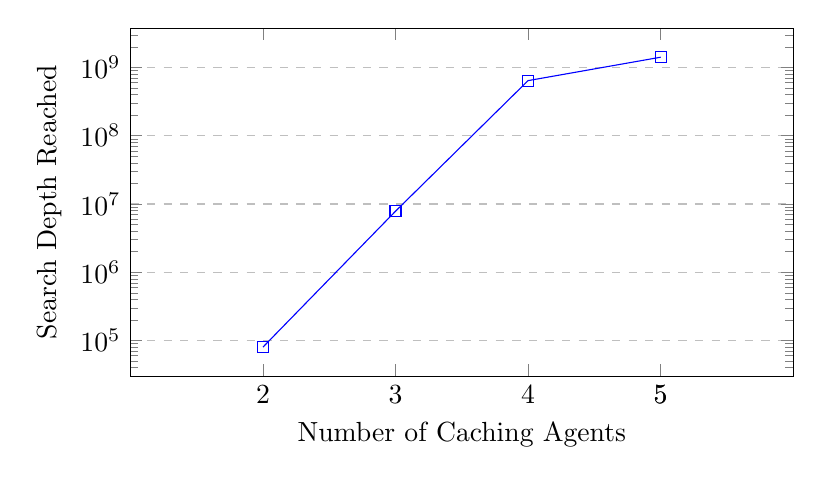
\begin{tikzpicture}
\begin{axis}[
    % title={Temperature dependence of CuSO\(_4\cdot\)5H\(_2\)O solubility},
    width=10cm,
    height=6cm,
    xlabel={Number of Caching Agents},
    ylabel={Search Depth Reached},
    xmin=1, xmax=6,
    %ymin=0, %ymax=120,
    xtick={2,3,4,5,5},
    % ytick={0,20,40,60,80,100,120},
    ymode=log,
    legend pos=north west,
    ymajorgrids=true,
    grid style=dashed,
]

\addplot[
    color=blue,
    mark=square,
    ]
    coordinates {
    (2,80051)(3,7832788)(4,640435248)(5,1410065407)
    };
    % \legend{CuSO\(_4\cdot\)5H\(_2\)O}
    
\end{axis}
\end{tikzpicture}
    \caption{Search depth reached during verification.}
    \label{fig:search-depth}
\end{figure*}

Configurations of 2, 3, and 4 caching agents have been successfully verified. Although one might initially assume that a protocol based on four states would have a small statespace this is not the reality. In fact, it is only possible to verify the MESI protocol for a small number of processors. The statespace grows astonishingly quickly. Each cache block has its own state information, each cache consists of multiple multiple cache blocks, each processor has its own cache and there is main memory above all the caches. Additionally, there are many intermediate states to handle communication between the processors and the web of transitions for each cache block. Statespace explosion is the greatest limiting factor for how large of a configuration can be verified. More specifically, verification is limited beyond 4 processors due to SPIN's max search depth of 1,410,065,407.

Even with significant effort invested in reducing the statespace, search depth, memory usage, and elapsed time grow by 2 orders of magnitude with each additional processor. Figure \ref{fig:search-depth} shows the maximum search depth reached versus number of caching agents. Figure \ref{fig:memory-usage} shows the memory used for storing states and additionally shows how compression improves as the number of caching agents increases. The time taken to verify each configuration is shown in Figure \ref{fig:verif-time} along with the rate at which the state space was being searched in states per second. With each additional processor there is a notable reduction in the rate of exploration.



\begin{figure*}
    \centering

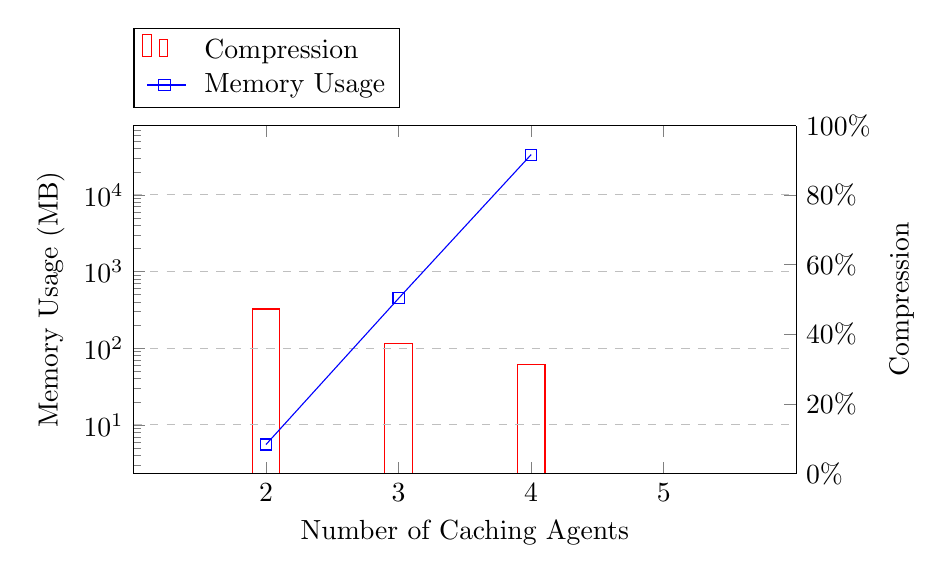
\begin{tikzpicture}
\begin{axis}[
      ybar,
      width  = 10cm,
      height = 6cm,
      hide x axis,
      axis y line*=right,
      xmin=1, xmax=6,
      ymin=0, ymax=100,
      % ytick={18,36,54, 72},
      ytick={0,20,40,60,80,100},
      ylabel={Compression},
      ylabel near ticks,
      yticklabel={\pgfmathparse{\tick*1}\pgfmathprintnumber{\pgfmathresult}\%},
      legend cell align=left,
      legend style={
                at={(0,1.05)},
                anchor=south west,
                column sep=1ex
      },
    ]

\addplot[
    color=red,
    % fill=red,
    ]
    coordinates {
    (2,47.29)(3,37.48)(4,31.41)(5,0)
    };
    \legend{Compression}
      \pgfplotsset{/pgfplots/line legend 2/.style={
legend image code/.code={\draw[-] (0cm,0cm)--(.5cm,0cm) node[midway, draw, regular polygon, regular polygon sides=4, minimum size=6pt, inner sep=0pt, xshift=-3pt] {};},},}
    \addlegendimage{line legend 2, blue}\addlegendentry{Memory Usage}
    % \legend{CuSO\(_4\cdot\)5H\(_2\)O}
\end{axis}
\begin{axis}[
    % title={Temperature dependence of CuSO\(_4\cdot\)5H\(_2\)O solubility},
    width=10cm,
    height=6cm,
    axis y line*=left,
    xlabel={Number of Caching Agents},
    ylabel={Memory Usage (MB)},
    xmin=1, xmax=6,
    %ymin=0, %ymax=120,
    xtick={2,3,4,5},
    % ytick={0,20,40,60,80,100,120},
    ymode=log,
    legend pos=north west,
    ymajorgrids=true,
    grid style=dashed,
]

\addplot[
    color=blue,
    mark=square,
    ]
    coordinates {
    (2,5.552)(3,446.803)(4,33516.065)(5,0)
    };
    % \legend{CuSO\(_4\cdot\)5H\(_2\)O}

\end{axis}
\end{tikzpicture}
    \caption{Actual memory usage for states and compression.}
    \label{fig:memory-usage}
\end{figure*}


\begin{figure*}
    \centering

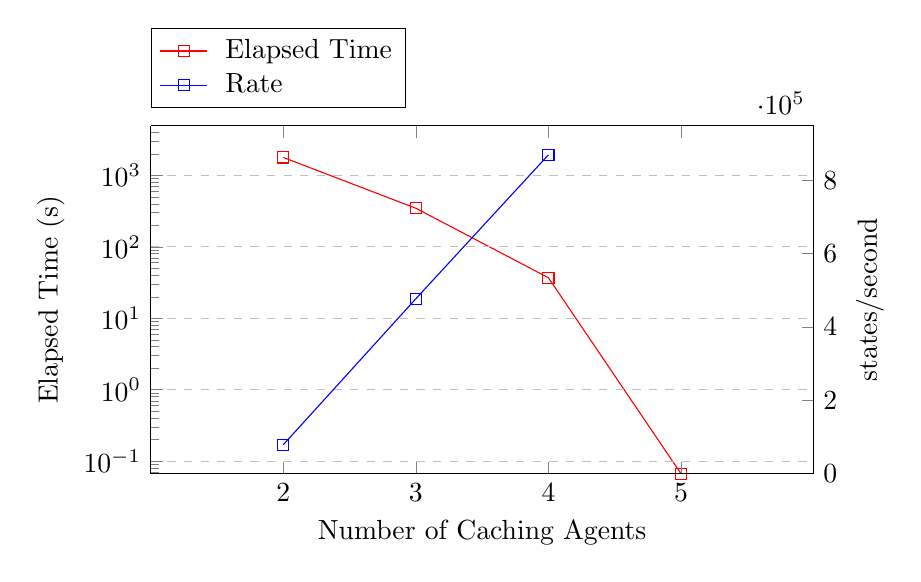
\begin{tikzpicture}
\begin{axis}[
      width  = 10cm,
      height = 6cm,
      hide x axis,
      axis y line*=right,
      xmin=1, xmax=6,
      ymin=0, %ymax=100,
      % ytick={18,36,54, 72},
      ylabel={states/second},
      legend cell align=left,
      legend style={
                at={(0,1.05)},
                anchor=south west,
                column sep=1ex
      },
    ]

\addplot[
    color=red,
    mark=square,
    ]
    coordinates {
    (2,862029.41)(3,723538.02)(4,534093.64)(5,0)
    };
    % \legend{CuSO\(_4\cdot\)5H\(_2\)O}
    \legend{Elapsed Time}
    \addlegendimage{blue, mark=square}\addlegendentry{Rate}

\end{axis}
\begin{axis}[
    % title={Temperature dependence of CuSO\(_4\cdot\)5H\(_2\)O solubility},
    width=10cm,
    height=6cm,
    axis y line*=left,
    xlabel={Number of Caching Agents},
    ylabel={Elapsed Time (s)},
    xmin=1, xmax=6,
    ymin=0, %ymax=120,
    xtick={2,3,4,5},
    % ytick={0,20,40,60,80,100,120},
    legend pos=north west,
    ymajorgrids=true,
    grid style=dashed,
    ymode=log,
]

\addplot[
    color=blue,
    mark=square,
    ]
    coordinates {
    (2,0.17)(3,18.8)(4,1940)(5,0)
    };
    % \legend{CuSO\(_4\cdot\)5H\(_2\)O} % seconds
    
    
\end{axis}
\end{tikzpicture}
    \caption{Verification time and rate.}
    \label{fig:verif-time}
\end{figure*}



\section{Conclusion} \label{conclusion}

The primary objective of this project is to verify the MESI Cache Coherency Protocol through \textit{Model Checking}. To this end, SPIN will be used to explore the state space and validate that the coherency property is not violated. There are a few additional considerations when creating the model. MESI is modular in the sense that it can be extended beyond the state space of just two caching-agents, with the practical limits being communication overhead and physical footprint of the processor. To verify as many configurations as possible, the number of caching agents $n$ as well as the cache size $m$ will be incremented until the state space becomes too large to model in SPIN. While the size of the caches could vary across caching-agents, in practice it is more common for caches at the same level to be symmetrical. This simplifies creating the model in SPIN and limits the number of configurations. Metrics such as memory usage and execution time of the SPIN verification will recorded so observations can be made about the impacts cache size and number of caching agents. To test that the model correctly represents the protocol, the resulting state space generated by SPIN will be compared to the calculated expected state space for each cache configuration. Furthermore, LTL specifications will be written to further test that each of the allowed transitions can occur, and that no disallowed transitions can occur.

All the code necessary to reproduce the results presented in this paper as well as the artifacts produced can be found on this project's github page: \href{https://github.com/IowaStateAerospaceCourses-Rozier/applied-formal-methods-final-project-cache-me-outside}{https://github.com/IowaStateAerospaceCourses-Rozier/applied-formal-methods-final-project-cache-me-outside}.

\clearpage{
\printbibliography
}

\end{document}
